Applikationen benytter tre Firebase produkter for at fungere, Authentication, Realtime Database og Storage.\\

 Firebase Auth\cite{FirebaseAuth} bruges til af håndtering brugere som login og oprettelse. Den indeholder data som Email, en hashet password og en unik identifier der bliver skabt af Firebase Authentication, når brugeren bliver skabt. Firebase tilbyder en Console , som er en web site, der giver mulighed at se og manipulere med sin data og konfigure sin Firebase.  Nedeunder kan et oversigt med informationer over brugerer ses. 
\begin{figure}[H] % (alternativt [H])
	\centering
	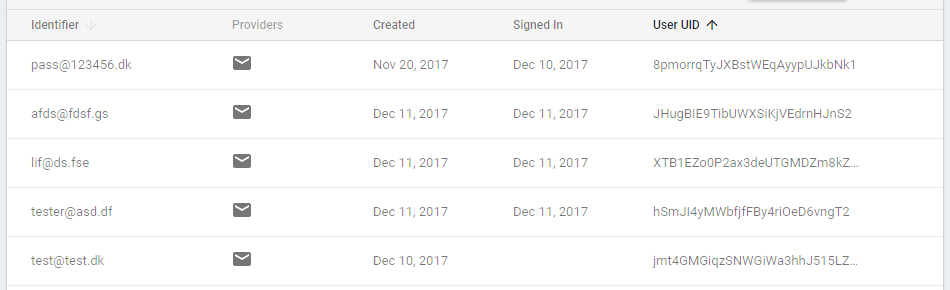
\includegraphics[height=5cm, width=15cm]{../ArkitekturDesign/Design/Firebase/FirebaseAuth.PNG}
	\caption{Oversigt over authentication data i firebase Console}
	\label{fig:FirebaseAuthPNG}
\end{figure}

Firebase Realtime Database bliver i forbindelse med applikationen vil blive brugt som en "opslagstavle", som vist nedeunder.  
 
\begin{figure}[H] % (alternativt [H])
	\centering
	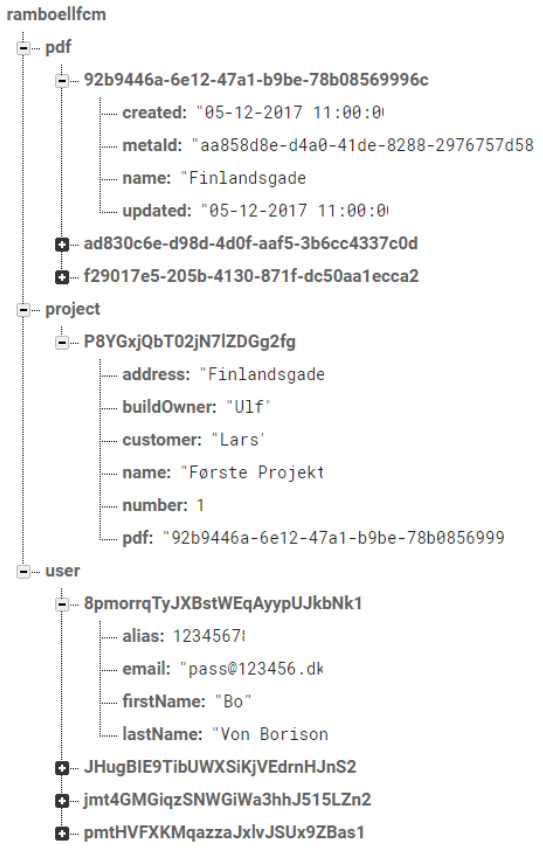
\includegraphics[height=10cm, width=10cm]{../ArkitekturDesign/Design/Firebase/FirebaseDB.PNG}
	\caption{Oversigt over database data i firebase Console}
	\label{fig:FirebaseDBPNG}
\end{figure}

På figur \ref{fig:FirebaseDBPNG} vises hvordan applikationens database er struktureret som et træ, med en root node\cite{rootNode} der hedder ramboellfcm, som derfra bliver opdelt i 3 noder pdf, project og user.
Pdf-node indeholder en liste af Guid \cite{GUID}, hvor hvert Guid har nogle ekstra informationer tilhørende den pågældende Guid, som for eksempel "metaId", hvilket er endnu en Guid, der peger på en json fil i Firebase Storage. Det samme har vi i project-node, som har en Guid der peger på en pdf-node. 
1
På den måde kan man let få en oversigt over hvilket projekter og 

